\documentclass{beamer}
\usetheme{Madrid}
\usecolortheme{default}
\useoutertheme{split}
\useinnertheme{circles}
\usepackage{xcolor}
\usepackage{mathrsfs}
\usepackage{amsmath}
\usepackage{amssymb}
\usepackage{booktabs}
\usepackage{hyperref}
\usepackage{animate}
\usepackage{caption}
\captionsetup[figure]{font=tiny}

\usepackage[
    backend=biber,
    style=alphabetic,
    sorting=ynt
]{biblatex}
\addbibresource{bibliography.bib}

% --- Couleurs CS ---
\definecolor{CSred}{RGB}{160,32,60}
\definecolor{CSgrey}{RGB}{136,121,150}
\definecolor{UPSred}{RGB}{97,21,58}
\setbeamercolor{titlelike}{bg=CSred}
\setbeamerfont{title}{series=\bfseries}
\setbeamercolor{palette primary}{bg=CSred,fg=white}
\setbeamercolor{palette secondary}{bg=CSred,fg=white}
\setbeamercolor{palette tertiary}{bg=CSgrey,fg=white}
\setbeamercolor{palette quaternary}{bg=CSgrey,fg=white}
\setbeamercolor{structure}{fg=CSgrey}

\title[Extreme Values]{Statistical Learning with Extreme Values}
\subtitle{Presentation - Paper Reading Assignment}
\author[Jamal, Basseras]{Adonis~JAMAL \and Théo~BASSERAS\\Sparse representation of multivariate extremes with
applications to anomaly detection}
\institute[ENS Paris-Saclay]{Ecole Normale Supérieure Paris-Saclay - MVA}
\date[December 18th 2025]{December 18th 2025}

\titlegraphic{
    
\includegraphics[height=1.2cm]{img/logo_mva.jpg}
}

\begin{document}

\frame{\titlepage}

% ==============================================================================
% SECTION 1: REAL WORLD PROBLEM
% ==============================================================================
\section{Context}
\begin{frame}{The "Crypto" Intuition: When is a Crash an Anomaly?}
    \textbf{The Scenario:}
    You manage a portfolio of 6 assets:
    \texttt{BTC}, \texttt{ETH}, \texttt{BNB}, \texttt{SOL}, \texttt{XRP}, and \texttt{USDT} (Stablecoin).
    
    \vspace{0.3cm}
    \textbf{Two types of Extreme Events:}
    \begin{columns}
        \column{0.48\textwidth}
        \begin{block}{Type A: Systemic Crash}
            \centering
            Bitcoin drops 20\%, everything else drops 20\%. \\
            \vspace{0.2cm}
            \textbf{Is this an anomaly?} \\
            \textcolor{CSred}{\textbf{NO.}} It's a standard market crash.
        \end{block}

        \column{0.48\textwidth}
        \begin{block}{Type B: The De-peg}
            \centering
            Bitcoin is stable, but \textbf{USDT} (Stablecoin) drops 20\%. \\
            \vspace{0.2cm}
            \textbf{Is this an anomaly?} \\
            \textcolor{green!50!black}{\textbf{YES.}} This is structural failure.
        \end{block}
    \end{columns}

    \vspace{0.3cm}
    \textbf{The Challenge:} Standard anomaly detection (Distance/Correlation) fails here because both events look "far from the mean." We need \textbf{Multivariate EVT}.
\end{frame}

% -------------------------------------------------------------------
% SLIDE 3: The Theory (Simplified)
% -------------------------------------------------------------------
\section{Theoretical Framework}
\begin{frame}{The Theoretical Barrier: The Curse of Dimensionality}
    \textbf{Goal:} Model the dependence of extremes (The Angular Measure $\Phi$).
    
    \begin{alertblock}{The Problem}
    \begin{itemize}
        \item In high dimensions ($d > 10$), the "sphere" of directions is too big.
        \item Data is sparse: We cannot estimate the density everywhere.
    \end{itemize}
    \end{alertblock}

    \textbf{The Solution (Goix et al., 2017) \cite{GOIX201712}: Sparsity Hypothesis}
    \begin{itemize}
        \item Extremes don't happen "everywhere" on the sphere.
        \item They concentrate on specific low-dimensional \textbf{sub-cones} (faces).
    \end{itemize}
    
    \vspace{0.3cm}
    \centering
    \textit{Intuition:} In our data, a crash of $\{BTC, ETH\}$ is common.\\ A crash of $\{BTC, USDT\}$ is physically unlikely.
\end{frame}

% -------------------------------------------------------------------
% SLIDE 4: Geometric Intuition
% -------------------------------------------------------------------
\section{Methodology}
\subsection{Approach}
\begin{frame}{Geometric Approach: $\epsilon$-Thickened Rectangles}
    \textbf{Problem:} Real data never lies \textit{exactly} on a lower-dimensional face.
    \vspace{0.2cm}

    \begin{columns}
        % Left Column: The Definition
        \column{0.5\textwidth}
            \begin{block}{Defining a "Cone" (Pattern)}
                An observation $x$ belongs to pattern $\alpha$ if:

                \textbf{Active ($j \in \alpha$):} Large ($> \epsilon \|x\|_\infty$)

                \textbf{Inactive ($j \notin \alpha$):} Small ($\le \epsilon \|x\|_\infty$)
            \end{block}

        \column{0.5\textwidth}
            \centering
            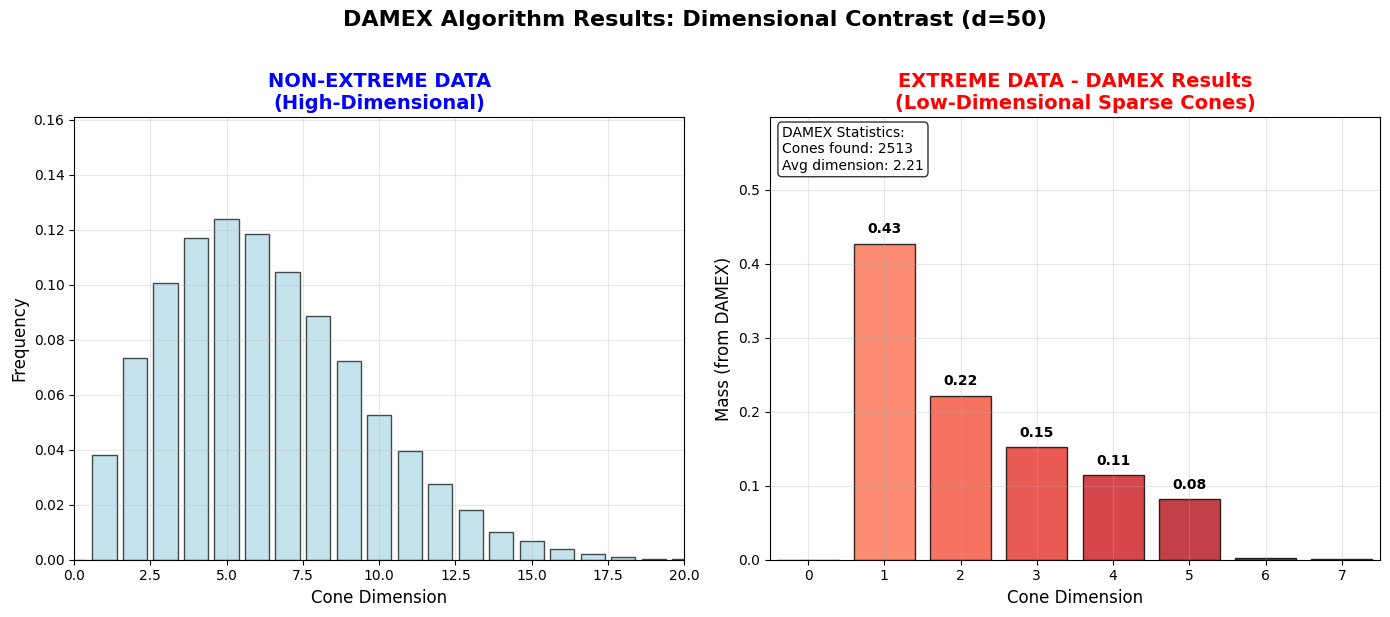
\includegraphics[width=\linewidth]{img/sparsity.png}
    \end{columns}

    \vspace{0.4cm}

    \textbf{The Estimator:} We count how many extreme points match this pattern.
    $$ \hat{\mathcal{M}}(\alpha) = \frac{1}{k} \sum_{i=1}^n \mathbb{I} \left\{ \text{Point } i \in \text{Cone } \alpha \cap \{R_i>n/k\} \right\} $$
    
    \small{\textit{Note: We apply a threshold to remove cones with negligible mass (noise).}}
\end{frame}

% -------------------------------------------------------------------
% SLIDE 5: The Algorithm
% -------------------------------------------------------------------
\subsection{Scoring Anomalies}
\begin{frame}{DAMEX: Detecting Anomaly with Multivariate EXtremes}
    \begin{enumerate}
        \item \textbf{Standardize:} Transform data to Pareto scale $$S_j(x) = \#\{X_i^j>x, i \leq n\}/n \quad V_i^j = 1/S_j(X_i^j)$$
        \item \textbf{Learn:} Estimate the mass $\hat{\mathcal{M}}(\alpha)$ for every cone (The "Normal" Profile).
        \item \textbf{Score:} For a new extreme point $x$:
    \end{enumerate}
    \vspace{-0.2cm}
    \begin{block}{The Anomaly Score}
        $$ s_n(x) \propto \frac{\text{Mass of the Cone containing } x}{\text{Magnitude of } x} $$
    \end{block}

    \begin{itemize}
        \item \textbf{Systemic Crash:} $x \in \{BTC, ETH, ...\}$. This cone has \textbf{High Mass}.
        $\Rightarrow$ Score is High (Normal Extreme).
        \item \textbf{De-peg:} $x \in \{BTC, USDT\}$. This cone has \textbf{Zero Mass}.
        $\Rightarrow$ Score is Low (Anomaly).
    \end{itemize}
\end{frame}

% -------------------------------------------------------------------
% SLIDE 7: Feature Clustering Methodology
% -------------------------------------------------------------------
\section{Results}
\subsection{Feature Clustering}
\begin{frame}{Feature Clustering Methodology}
    
\textbf{Goal:} Find features with similar behavior on extreme data.
\vspace{0.2cm}
\begin{columns}
    \column{0.6\textwidth}
    \textbf{Dependence test} (cluster $A = \{i, j, k\}$, extreme data only):
    \[H_0: P(\text{Ex}) = \prod P(\text{Ex}_i)\]
    \[H_1: P(\text{Ex}) > \prod P(\text{Ex}_i)\]

    \textbf{Optimization:} Use DAMEX cones, minimize:\\$\text{AIC} = \text{Training Deviance} + 2 \times \frac{\# \text{subfaces}}{n_{\text{extremes}}}$

    \column{0.4\textwidth}
    \centering
    \begin{figure}[h]
        \centering
        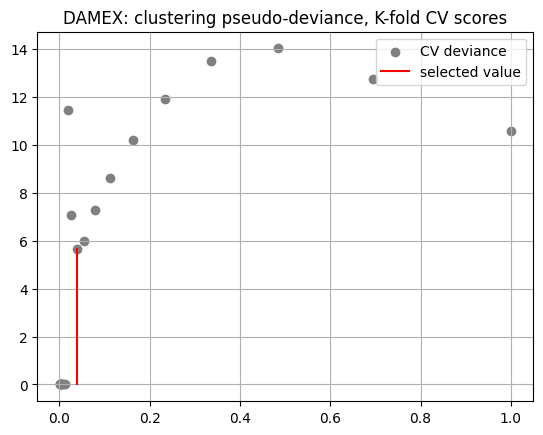
\includegraphics[width=\textwidth]{img/AIC_eps.png}
        \caption{AIC vs $\epsilon$: 1) Null model, 2) Optimal, 3) Overfit, 4) Double descent}
        \label{pseudo_deviance}
    \end{figure}
\end{columns}
\end{frame}

% -------------------------------------------------------------------
% SLIDE 6: Results (The Case Study)
% -------------------------------------------------------------------
\subsection{Crypto Crash Structure}
\begin{frame}{The Structure of Crypto Crashes}
    We applied DAMEX to daily returns (2020-2024). 
    \textbf{What "Normal" extremes did it find?}

    \begin{table}[]
        \centering
        \footnotesize
        \begin{tabular}{llc}
            \toprule
            \textbf{Cone Type} & \textbf{Assets Involved} & \textbf{Mass (Likelihood)} \\
            \midrule
            \textbf{1. Systemic} & \texttt{BTC + ETH + BNB + SOL + XRP} & \textbf{1.00} \\
            & \textit{(The whole market moves together)} & \\
            \midrule
            \textbf{2. Idiosyncratic} & \texttt{USDT} (Stablecoin) & \textbf{0.72} \\
            & \textit{(Stablecoin volatility is isolated)} & \\
            \midrule
            \textbf{3. Noise} & \texttt{SOL + USDT} & \textbf{0.18} \\
            & \textit{(Rare/Weak dependence)} & \\
            \bottomrule
        \end{tabular}
    \end{table}

    \textbf{Finding:} The algorithm successfully "decoupled" the Stablecoin from the speculative assets without supervision.
\end{frame}

% -------------------------------------------------------------------
% SLIDE 8: Conclusion
% -------------------------------------------------------------------
\section{Conclusion}
\subsection{Conclusion}
\begin{frame}{Conclusion}
    \textbf{Summary:}
    \begin{enumerate}
        \item \textbf{Sparsity is key:} In high dimensions, extremes concentrate on low-dimensional faces (sub-groups).
        \item \textbf{Geometry over Magnitude:} Anomalies in the tail are defined by \emph{directions} ($\epsilon$-cones), not just distance.
        \item \textbf{Practical Value:} DAMEX allows risk managers to distinguish "Panic Selling" (Systemic) from "Asset Failure" (Structural).
    \end{enumerate}

    \vspace{0.5cm}
    \textbf{Future Work:}
    \begin{itemize}
        \item Selecting $\epsilon$ and $k$ is hard. We implemented an AIC criterion (see report) to automate this.
    \end{itemize}
\end{frame}

% ==============================================================================
% SECTION : BIBLIOGRAPHY
% ==============================================================================
\subsection{Bibliography}
\begin{frame}[allowframebreaks]{Bibliography}
    \frametitle{Bibliography}
    \printbibliography[heading=none]
\end{frame}

% ==============================================================================
% SECTION : APPENDIX
% ==============================================================================
\subsection{Appendix}
\begin{frame}{Appendix}
   
\end{frame}


\end{document}